\section{Results}
\label{sec:results}

\subsection{X particles reconstruction efficiency}
\label{subsec:signalefficiency}

The signal events contain two \X bosons decaying to \qq, therefore we define the \X bosons 
 efficiency times acceptance ($\epsilon A$) as:
\begin{equation}
\epsilon A= \frac{N_{X reconstructed}}{2N_{events}}
\end{equation}

where the X bosons acceptance $A$ has been defined in Section \ref{subsec:sigsensitivity}. 
Table \ref{tab:sigeff} presents the acceptance and efficiency for
reconstructing \X boson candidates as a function of the \Higgs and \X particles masses for different 
mean lifetimes of the \X particles.

\begin{table}[htbp]
\caption{Signal reconstruction efficiency for individual $\X\rightarrow\qq$ decays in simulated signal models. 
Both trigger and reconstruction efficiency 
are included in the calculation. Uncertainties quoted on signal efficiencies are statistical only.\label{tab:sigeff}}
\centering
\begin{tabular}{lllll} 
\hline
$H^{0}$ [GeV] & $X$ [GeV] & c$\tau$ [cm] & Acceptance [\%] & $\epsilon$ [\%] \\
\hline
200 & 50 & 2 & $8.9\pm0.2$ & $1.5\pm0.3$ \\
200 & 50 & 20 & $7.2\pm0.2$ & $0.8\pm0.2$ \\
\hline
400 & 50 & 0.8 & $35.0\pm0.4$ & $8.9\pm0.4$ \\
400 & 50 & 8 & $31.0\pm0.4$ & $4.5\pm0.3$ \\
400 & 50 & 80 & $7.1\pm0.2$ & $1.6\pm0.4$ \\
\hline
400 & 150 & 4 & $59.0\pm0.4$ & $16.0\pm0.4$ \\
400 & 150 & 40 & $50.0\pm0.4$ & $6.9\pm0.3$ \\
400 & 150 & 400 & $13.0\pm0.3$ & $1.8\pm0.3$ \\
\hline
1000 & 150 & 1 & $73.0\pm0.4$ & $38.0\pm0.4$ \\
1000 & 150 & 10 & $66.0\pm0.4$ & $26.0\pm0.4$ \\
1000 & 150 & 100 & $15.0\pm0.3$ & $15.0\pm0.7$ \\
\hline
1000 & 350 & 3.5 & $87.0\pm0.3$ & $40.0\pm0.4$ \\
1000 & 350 & 35 & $76.0\pm0.3$ & $22.0\pm0.4$ \\
1000 & 350 & 350 & $19.0\pm0.3$ & $11.0\pm0.5$ \\
\hline
\end{tabular} 
\end{table}

\X particle reconstruction efficiencies presented in Table \ref{tab:sigeff} 
are applicable to a model where \X particles decay with equal branching fractions to u,d,s,c and b quark pairs.
Table \ref{tab:sigeffflavor} shows the \X particle reconstruction efficiencies separately for 
\X decaying light quarks (u,d,s) and
heavier quarks c and b. 


\begin{table}[htbp]
\caption{Signal reconstruction efficiency for individual $\X\rightarrow\qq$ decays
 in simulated signal models for light (uds) and heavy (c and b) quark flavors.
 Uncertainties quoted on signal efficiencies are statistical only.\label{tab:sigeffflavor}} 
\centering 
\begin{tabular}{llllll} 
\hline
$H^{0}$ [GeV] & $X$ [GeV] & c$\tau$ [cm] & $\epsilon_{uds}$ [\%] & $\epsilon_{c} [\%] $ & $\epsilon_{b}$ [\%]\\
\hline
200 & 50 & 2 & $1.9\pm0.4$ & $1.3\pm0.6$ & $0.5\pm0.4$ \\
200 & 50 & 20 & $0.92\pm0.3$ & $0.7\pm0.5$ & $0.5\pm0.4$ \\
\hline
400 & 50 & 0.8 & $10.0\pm0.5$ & $8.6\pm0.8$ & $4.2\pm0.6$ \\
400 & 50 & 8 & $5.3\pm0.4$ & $4.0\pm0.6$ & $2.5\pm0.5$ \\
400 & 50 & 80 & $1.9\pm0.5$ & $1.3\pm0.7$ & $0.92\pm0.6$ \\
\hline
400 & 150 & 4 & $18.0\pm0.5$ & $16.0\pm0.8$ & $11.0\pm0.7$ \\
400 & 150 & 40 & $7.5\pm0.4$ & $6.5\pm0.6$ & $5.4\pm0.5$ \\
400 & 150 & 400 & $2.1\pm0.4$ & $1.5\pm0.6$ & $1.2\pm0.5$ \\
\hline
1000 & 150 & 1 & $39.0\pm0.5$ & $39.0\pm0.9$ & $35.0\pm0.9$ \\
1000 & 150 & 10 & $26.0\pm0.5$ & $26.0\pm0.9$ & $25.0\pm0.9$ \\
1000 & 150 & 100 & $15.0\pm0.9$ & $16.0\pm2.0$ & $13.0\pm1.0$ \\
\hline
1000 & 350 & 3.5 & $41.0\pm0.5$ & $40.0\pm0.9$ & $36.0\pm0.8$ \\
1000 & 350 & 35 & $23.0\pm0.5$ & $22.0\pm0.8$ & $21.0\pm0.8$ \\
1000 & 350 & 350 & $12.0\pm0.7$ & $11.0\pm1.0$ & $9.4\pm1.0$ \\
\hline
\end{tabular} 
\end{table}

\begin{figure}[htbp]
\centering
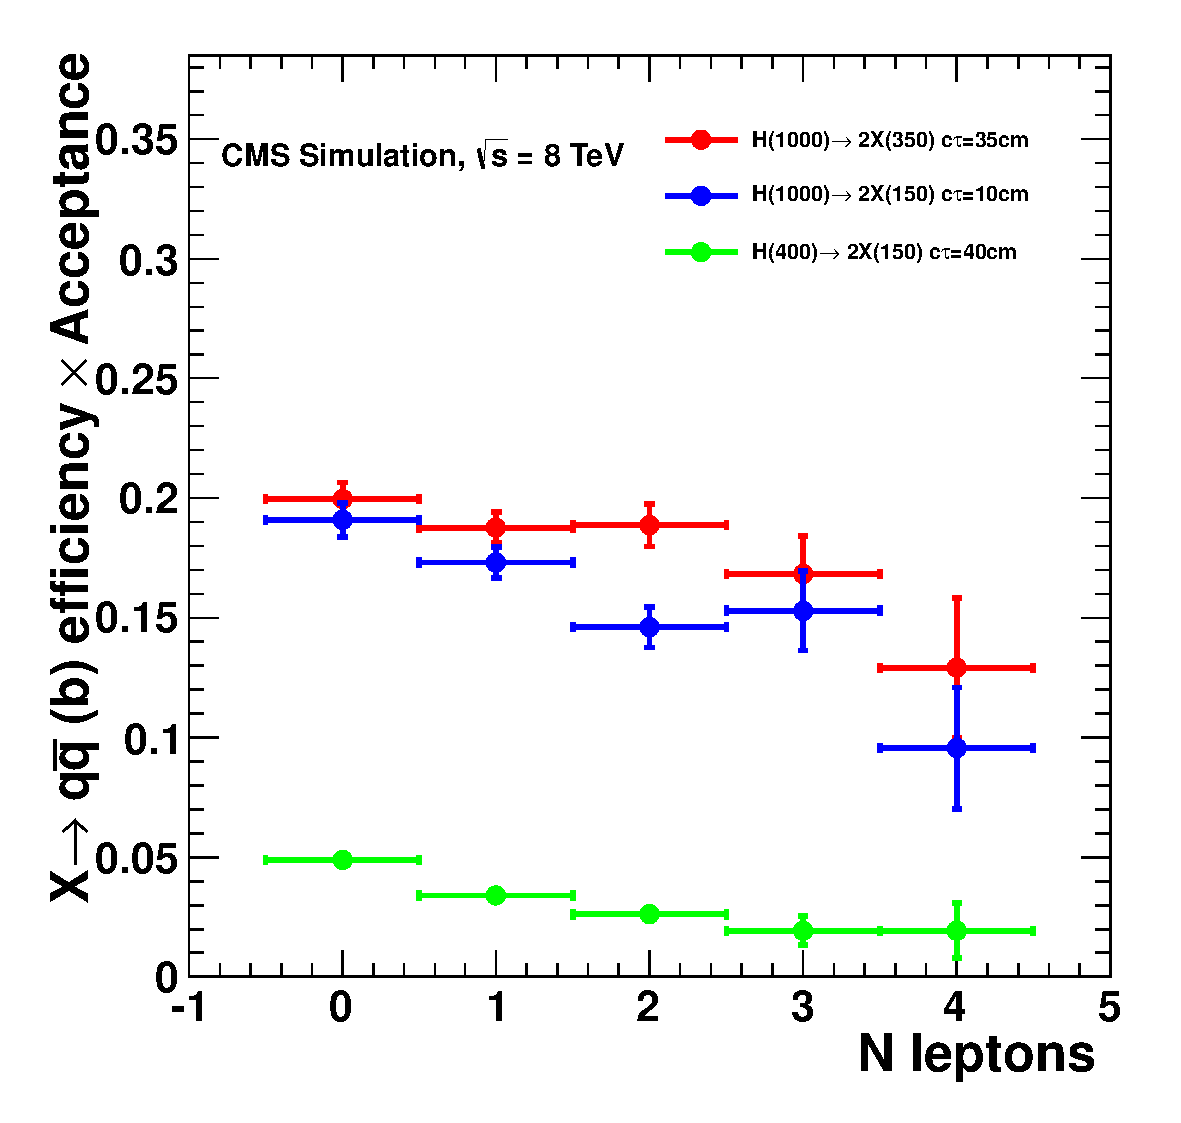
\includegraphics[width=0.49\textwidth]{plots/signal/effNLepb.pdf}
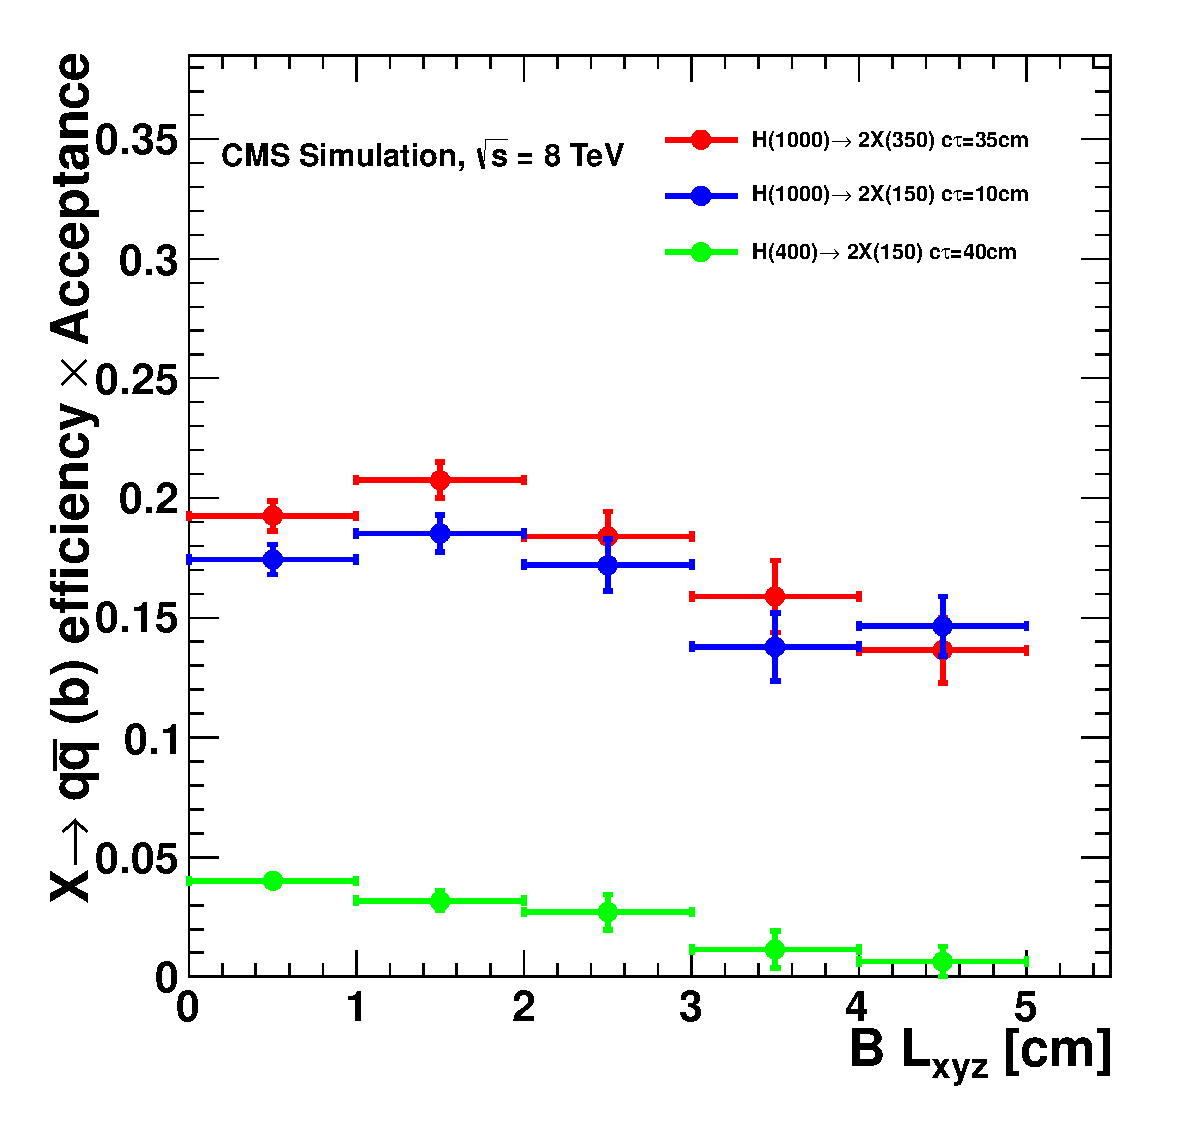
\includegraphics[width=0.49\textwidth]{plots/signal/effBlxyzb.pdf}
\caption{$\X\rightarrow b\bar{b}$ reconstruction efficiency as a function of the total number of leptons 
originating from B mesons/baryons (left) and as a function of B mesons/baryons decay length. Only selected 
mass points are shown. The samples correspond to the mixture of the three generated mean 
lifetimes of the \X bosons. \label{fig:effb}}
\end{figure}

The c and b quarks hadronize mostly into D or B mesons respectively.
 Unlike the light quark mesons a significant fraction of heavy flavor
mesons decays semi-leptonically reducing the track multiplicity of the jets and also reducing the jet momenta
 due to the missing energy of associated neutrinos. 
Additionally the D or B mesons split the dijet vertex due to their intrinsic lifetime.
Figure \ref{fig:effb} shows the reconstruction efficiency of the $\X\rightarrow b\bar{b}$ candidates as a function
of the total number of leptons originating from the $b\bar{b}$ pair and as a function of the B mesons decay
length. The reconstruction efficiency is affected mostly by the number of leptons, while the dependence on the
B mesons decay length is much smaller.

In order to visualize the capabilities of the CMS detector for reconstructing long-lived particles decaying to 
dijets, 
the reconstructed dijet mass and $L_{xy}$ distributions for selected signal models are shown in Figure
\ref{fig:signal}. We assume the cross-section of the $\Higgs\rightarrow2\X$ process to be 1 pb and the branching 
ratio to quarks ($\X\rightarrow\qq$) to be 100\%.

\begin{figure}[htbp]
\centering
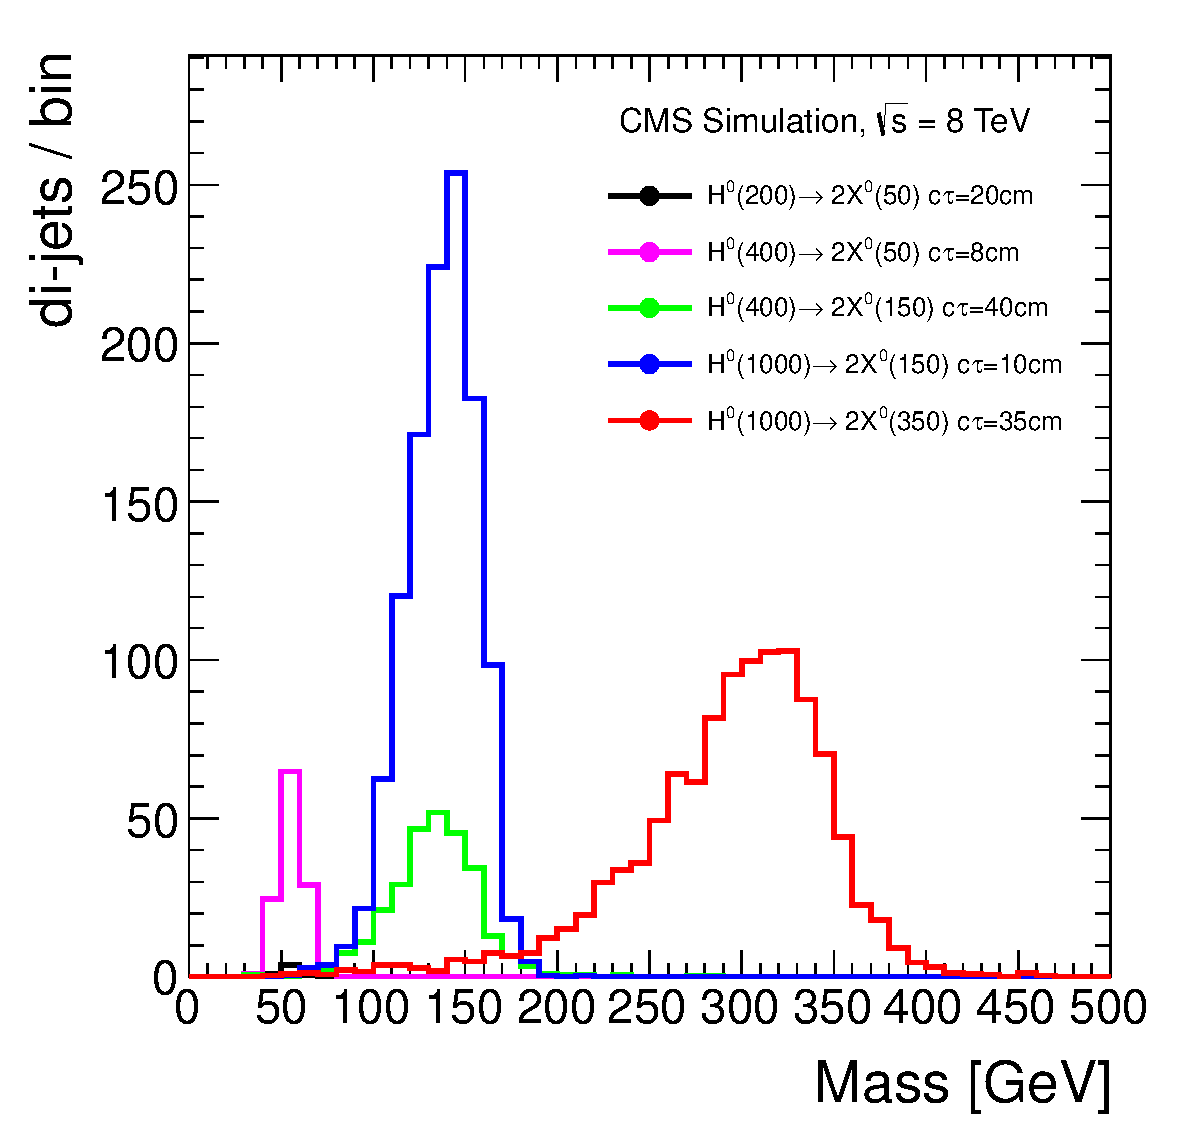
\includegraphics[width=0.49\textwidth]{plots/signal/mass.pdf}
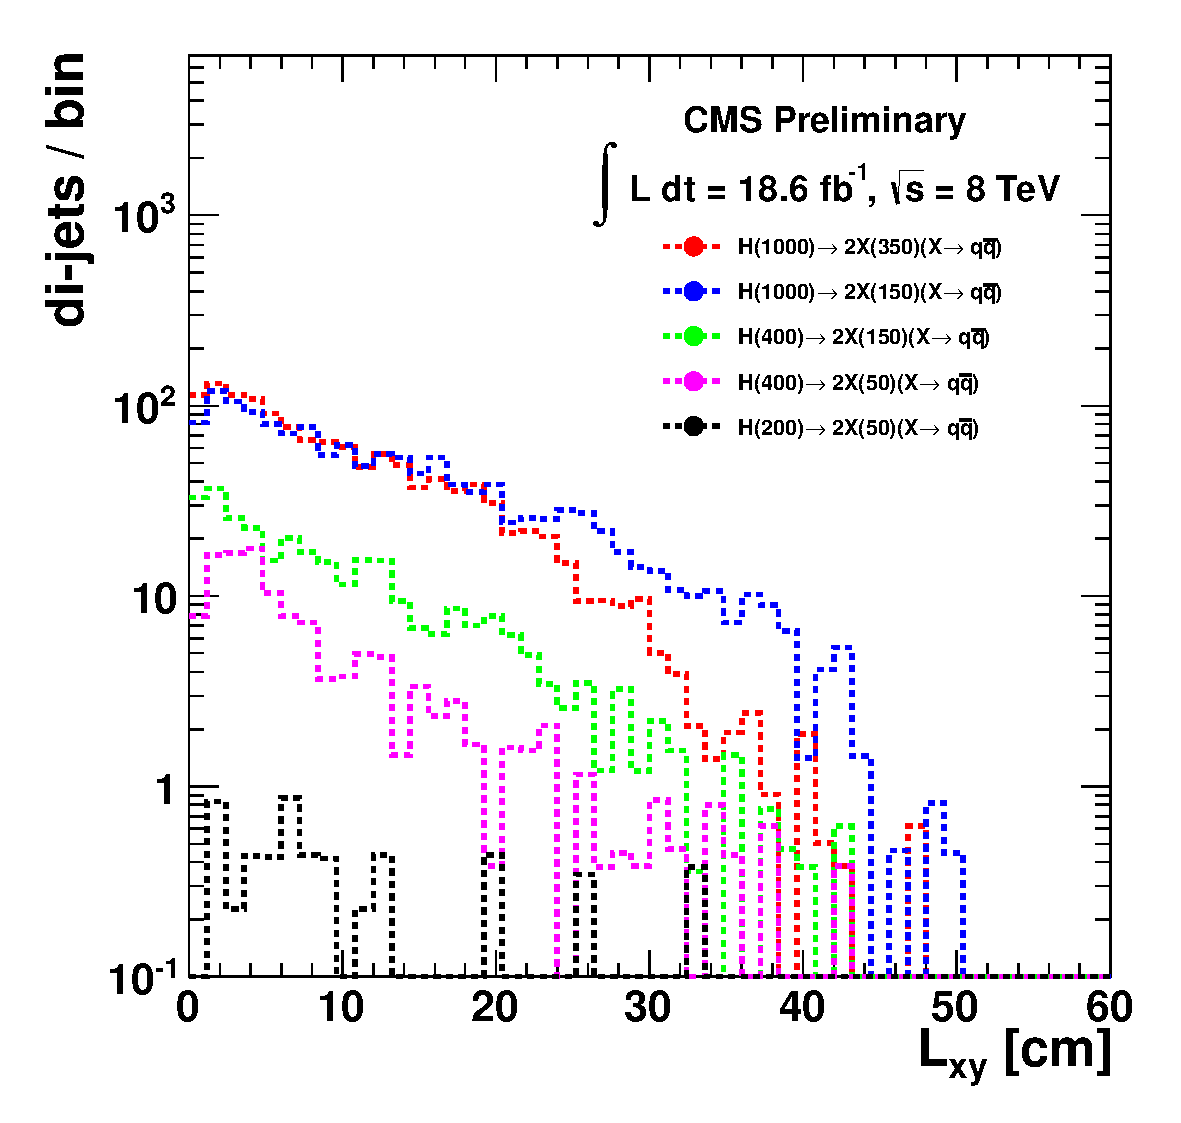
\includegraphics[width=0.49\textwidth]{plots/signal/Lxy.pdf}
\caption{The reconstructed dijet mass and $L_{xy}$ for selected signal models; central lifetime out of the three available is presented.\label{fig:signal}}
\end{figure}

\subsection{Data in the signal region}
\label{subsec:fullunblinding}

Table \ref{tab:fullunblinding} summarizes the observed candidate counts in the signal region for the optimized 
selections detailed in Section \ref{subsec:cutvalues}. Data is found in good agreement with the 
background only hypothesis. In addition, the two selected candidates are examined using event displays
and are found consistent with background candidates as described in Figure \ref{fig:eventDisplays}.  

\begin{table}[htbp]
\centering
\begin{tabular}{|l|c|c|}
\hline
$\bf L_{xy}$ \bf selection & \bf low & \bf high \\
\hline
\bf Predicted Background & $ 1.60\pm0.58(stat+sys)$ & $ 1.14\pm0.54(stat+sys)$ \\
\hline
\bf Observed candidates & 2 & 1 \\ 
\hline
\end{tabular}
\caption{Observed candidates and predicted background for the optimized selections.\label{tab:fullunblinding}}
\end{table}

\begin{figure}
\centering
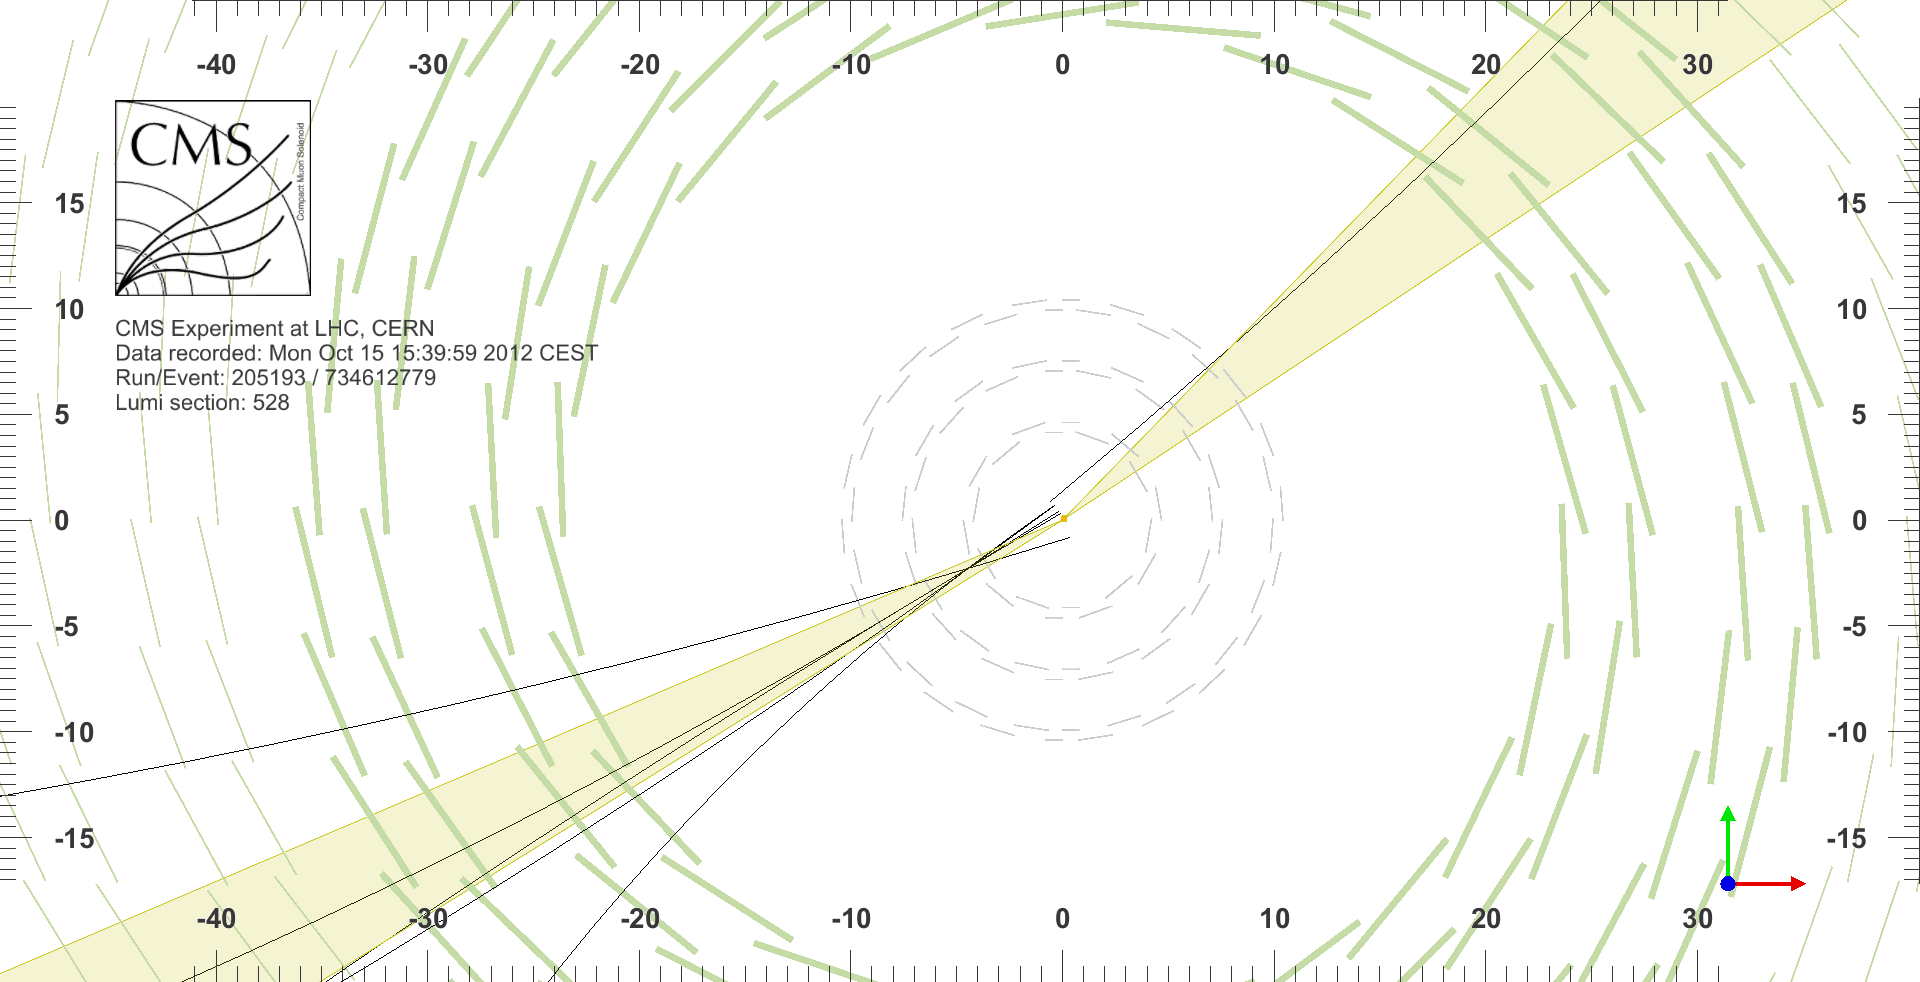
\includegraphics[width=0.495\textwidth]{plots/displays/ev1_vtx.png}
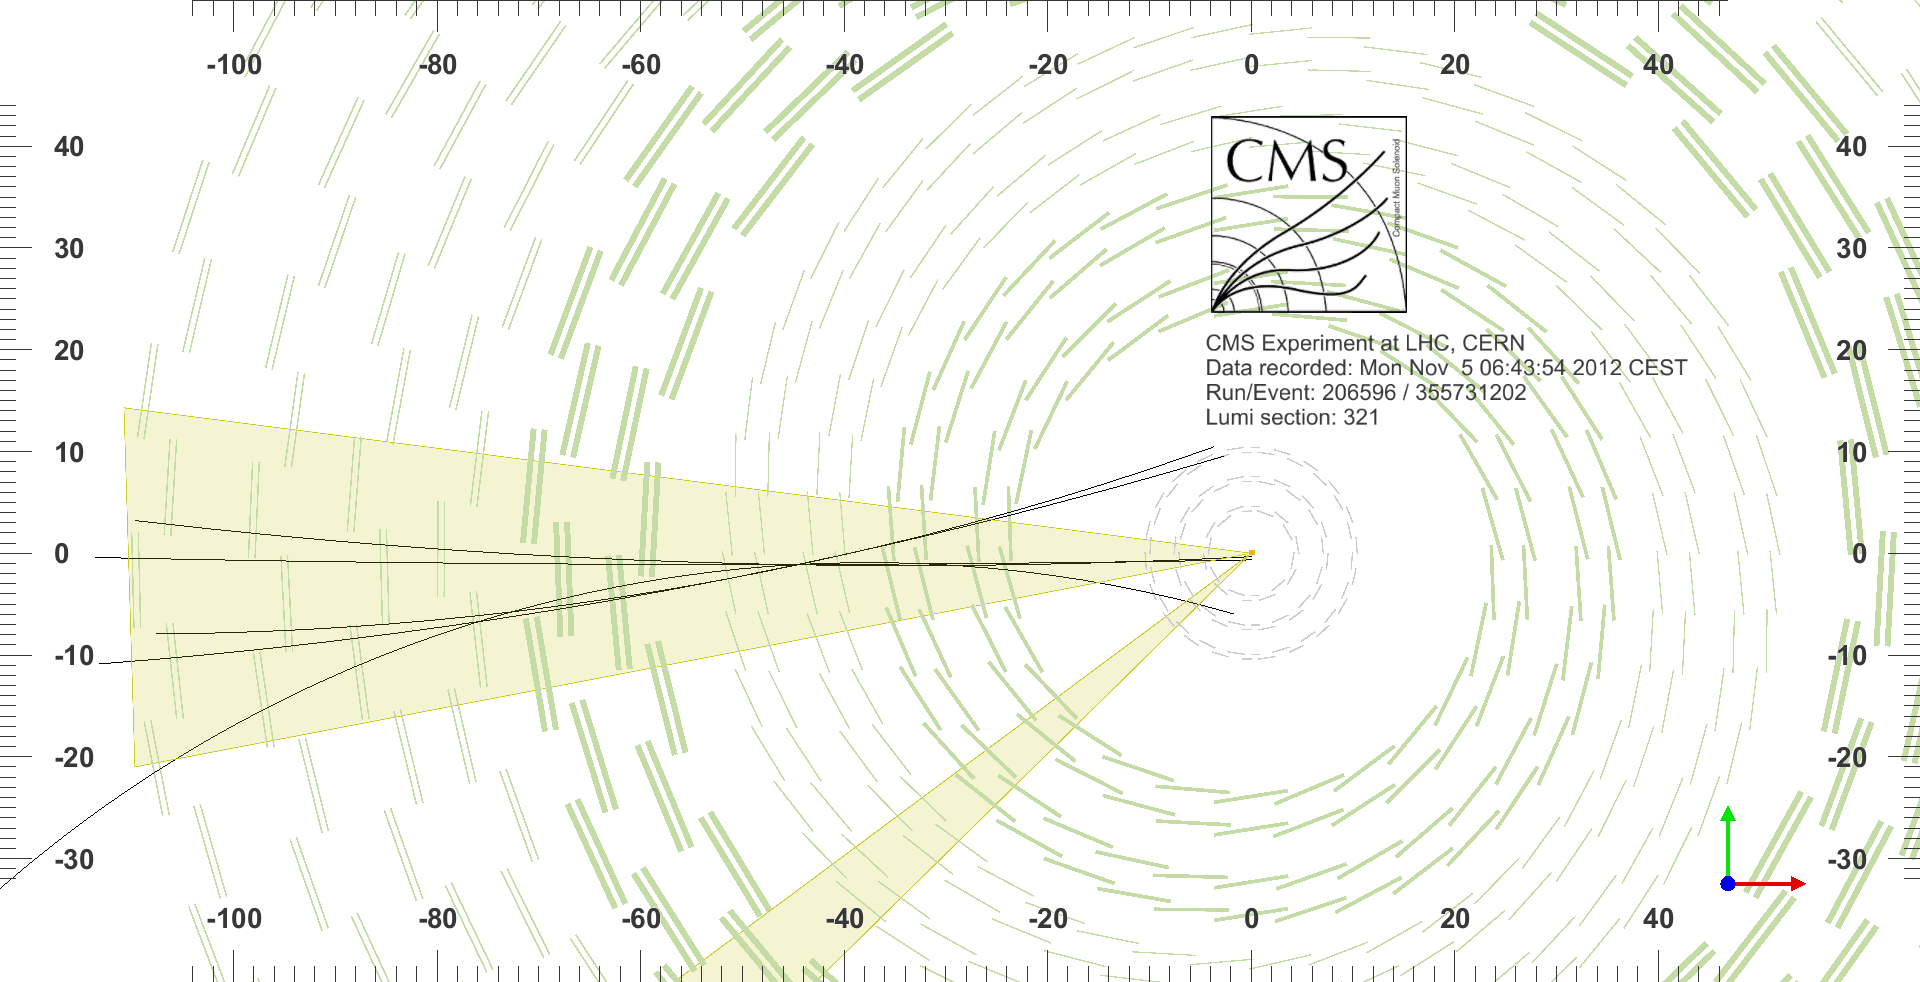
\includegraphics[width=0.495\textwidth]{plots/displays/ev2_vtx.png}

\caption{Event displays of the two candidates passing the optimized selection where only the selected di-jet pair
 (yellow cones) and 
the tracks associated to the displaced vertex (black lines) are shown, other objects being removed. 
Candidate 1 (left) with dijet invariant mass of 770 \GeVcc, which 
passes only the {\it low $L_{xy}$} selection, 
contains a secondary vertex, displaced transversely by 5 \cm, containing 5 tracks from one jet and 1 track
from the other. The 5 track vertex is consistent with a vertex of a B meson with invariant mass below 5 \GeVcc.
Candidate 2 (right) with dijet invariant mass of 75\GeVcc, 
which passes both {\it low} and {\it high $L_{xy}$} selections, contains a secondary vertex
, displaced transversely by 44 \cm, containing 5 tracks where 2 of these tracks are
associated to both jets due to the jets being nearby. The vertex invariant mass is low and its position
 coincides with one of the silicon 
tracker layers being consistent with a nuclear interaction vertex. \label{fig:eventDisplays}}
\end{figure} 



\subsection{Limits}
\label{subsec:limits}

Given the null result of the search an upper limit is quoted on the cross-section 
to produce $\Higgs\rightarrow \X\X$ times the branching ratio squared, $B^2$, for \X to decay into \qq. 
The expected number of signal dijet candidates passing the selection cuts can be expressed as:
\begin{equation}
N_X \geq 2 \mathcal{L}\epsilon A\sigma B^2
\end{equation}
where $\mathcal{L}$ is the integrated luminosity, $A$ is the acceptance,
 $\epsilon$ is the efficiency to reconstruct \X boson candidates
(Table \ref{tab:sigeff}), $\sigma$ is the production cross-section of the heavy resonance decaying to \XX and 
$B$ is the branching ratio of \X to dijets. The non-equality arises from the fact that when the branching ratio $B$
is smaller than 1, there is an additional contribution from events where only one \X boson decayed to dijets. 
The limits will therefore be exact when $B=1$ and conservative when $B$ is smaller than 1.
 

For each combination of the \Higgs and \X boson masses that are modelled and for a range of \X boson lifetimes,
the 95\% CL upper limits on $\sigma B^2$ are calculated.
  
%The lifetime re-weighting procedure is explained in Appendix \ref{sec:reweighting}.
 The limit calculation employs CL$_s$ method \cite{Read:2002hq} for a counting
experiment with 95\% confidence level. The calculation uses the statistics software 
package {\tt RooStatsCL95} recommended by
 the CMS Statistics Committee \cite{RooStatsCL95}. 

In order to expand the number of tested models
the lifetime distributions of the signal MC events are re-weighted to different
mean values using generator level lifetimes, thus providing additional signal efficiencies. 
%The lifetime re-weighting procedure is explained in Appendix \ref{sec:reweighting}.
The limits on $\sigma B^2$ and the limits on $\sigma B^2 A$ corrected for detector acceptance are computed. 
They are presetned in Figures
\ref{fig:limits} and \ref{fig:limitsacceptance} respectively.

\begin{figure}[htbp]
\centering
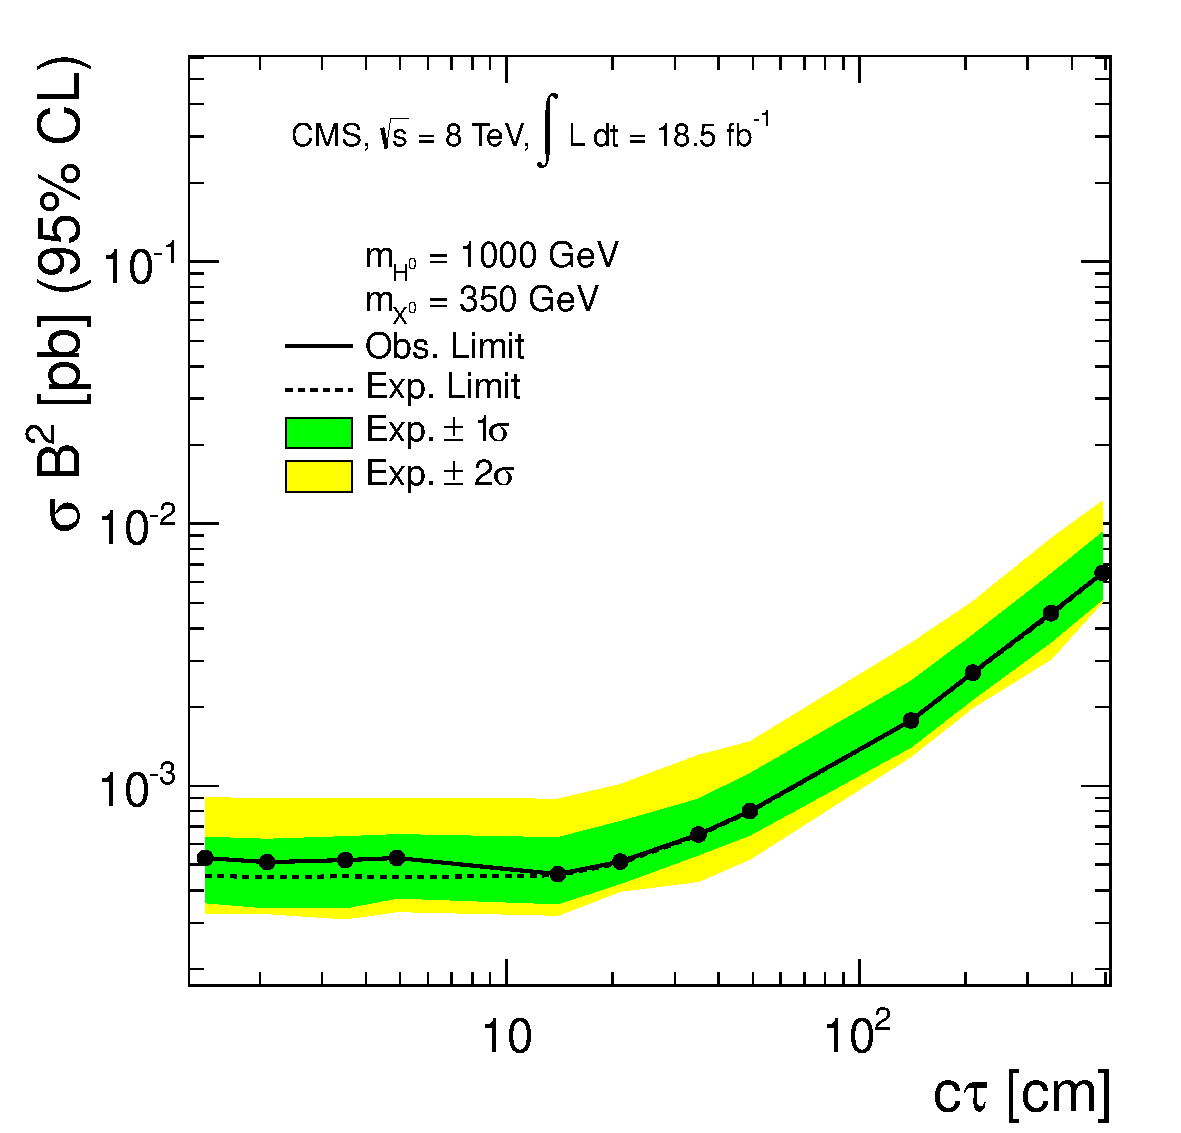
\includegraphics[width=0.49\textwidth]{plots/limits/1000_350e.pdf}
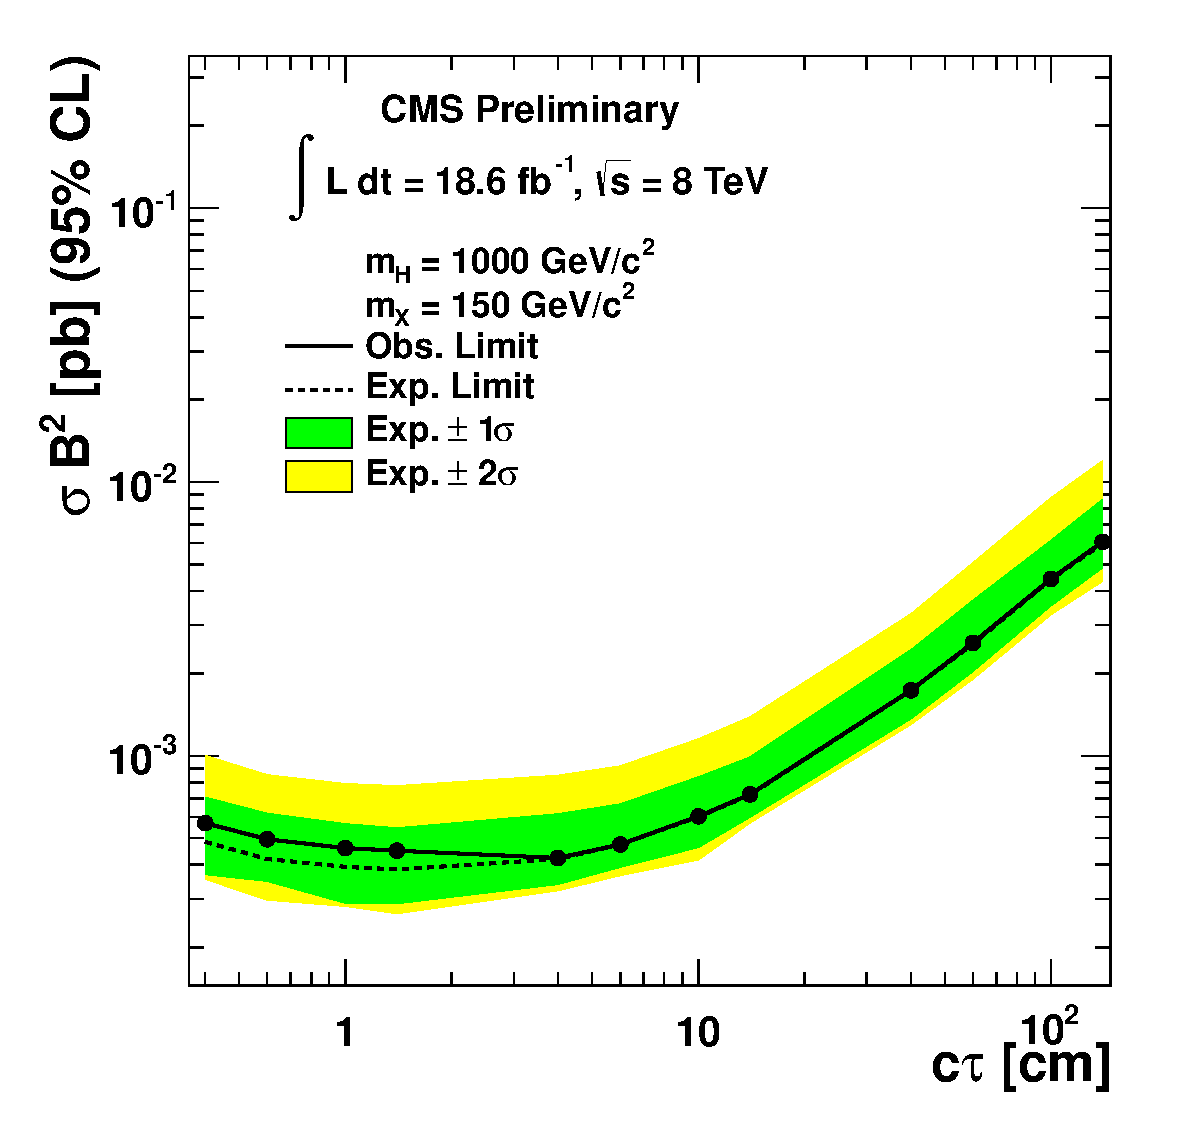
\includegraphics[width=0.49\textwidth]{plots/limits/1000_150e.pdf} 
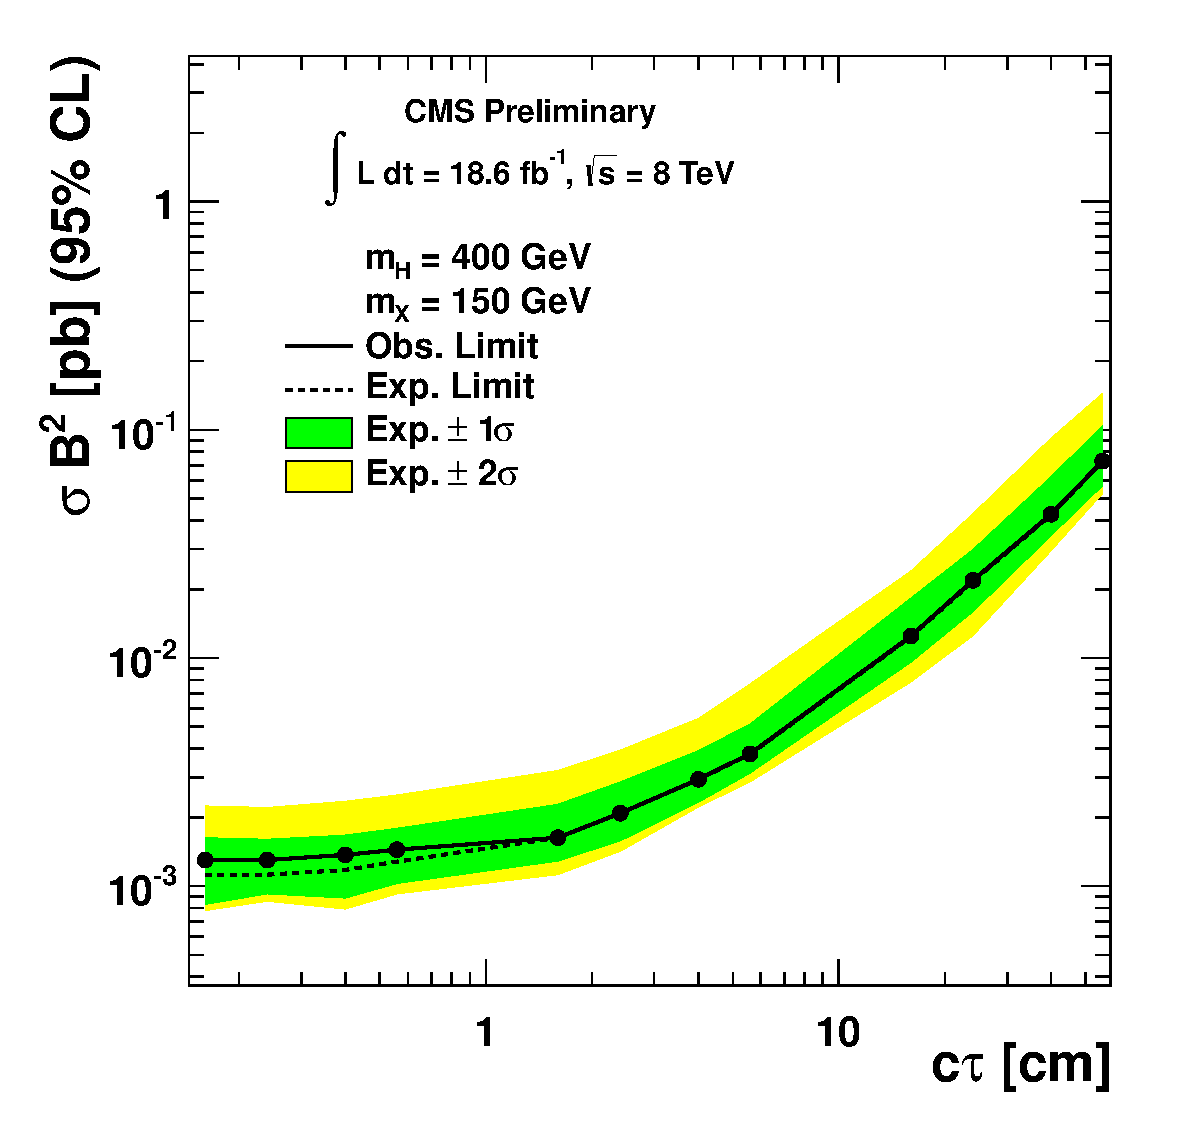
\includegraphics[width=0.49\textwidth]{plots/limits/400_150e.pdf}
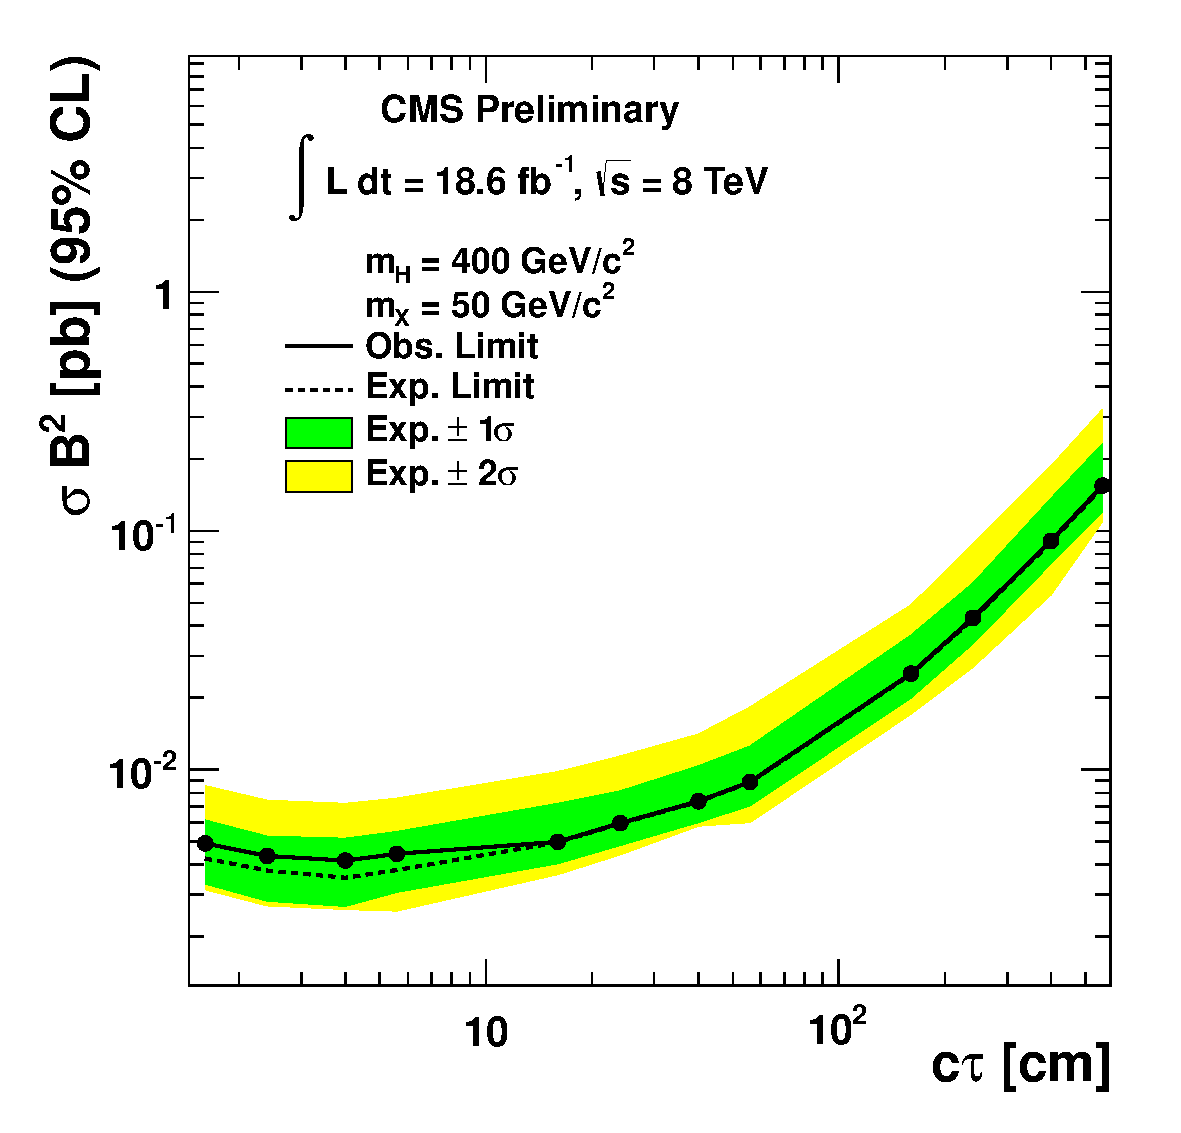
\includegraphics[width=0.49\textwidth]{plots/limits/400_50e.pdf} 
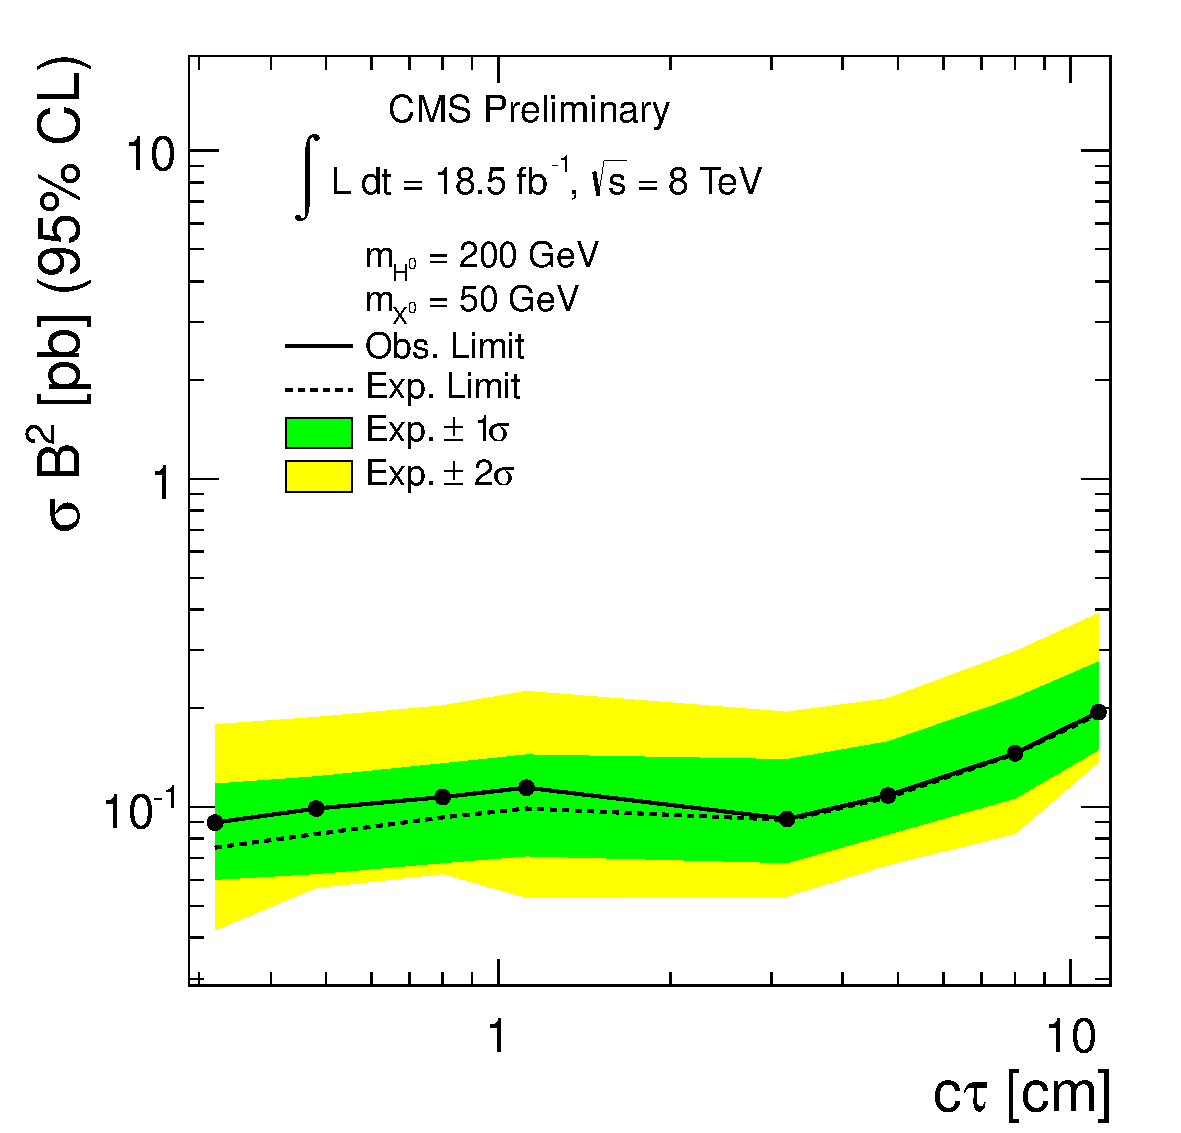
\includegraphics[width=0.49\textwidth]{plots/limits/200_50e.pdf}

\caption{Expected and observed 95\% CL limits for all tested signal models.\label{fig:limits}}
\end{figure}

\begin{figure}[htbp]
\centering
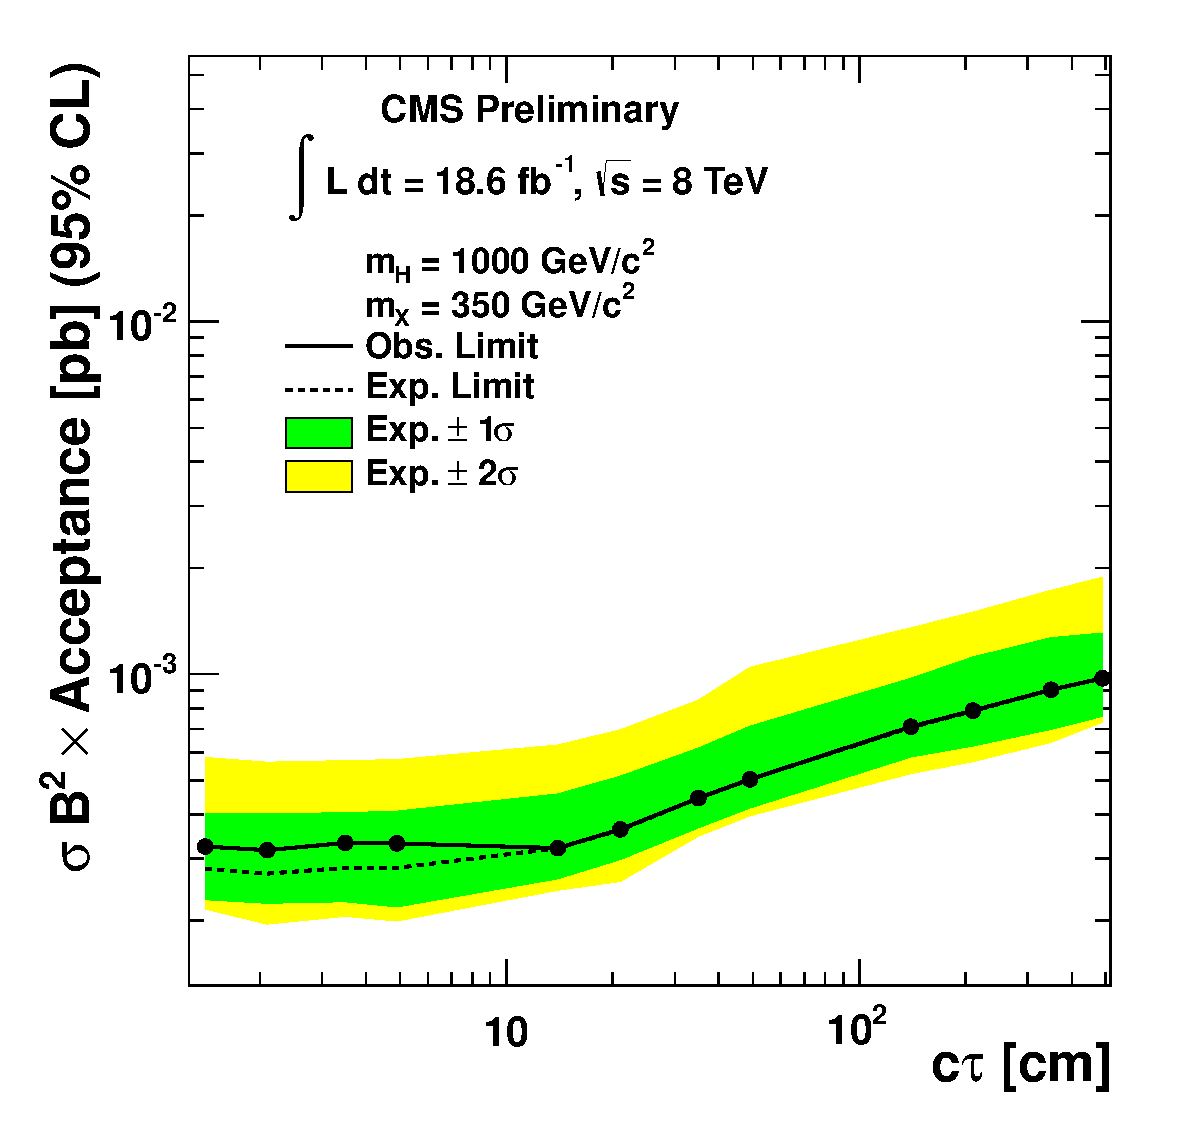
\includegraphics[width=0.49\textwidth]{plots/limits/1000_350ea.pdf}
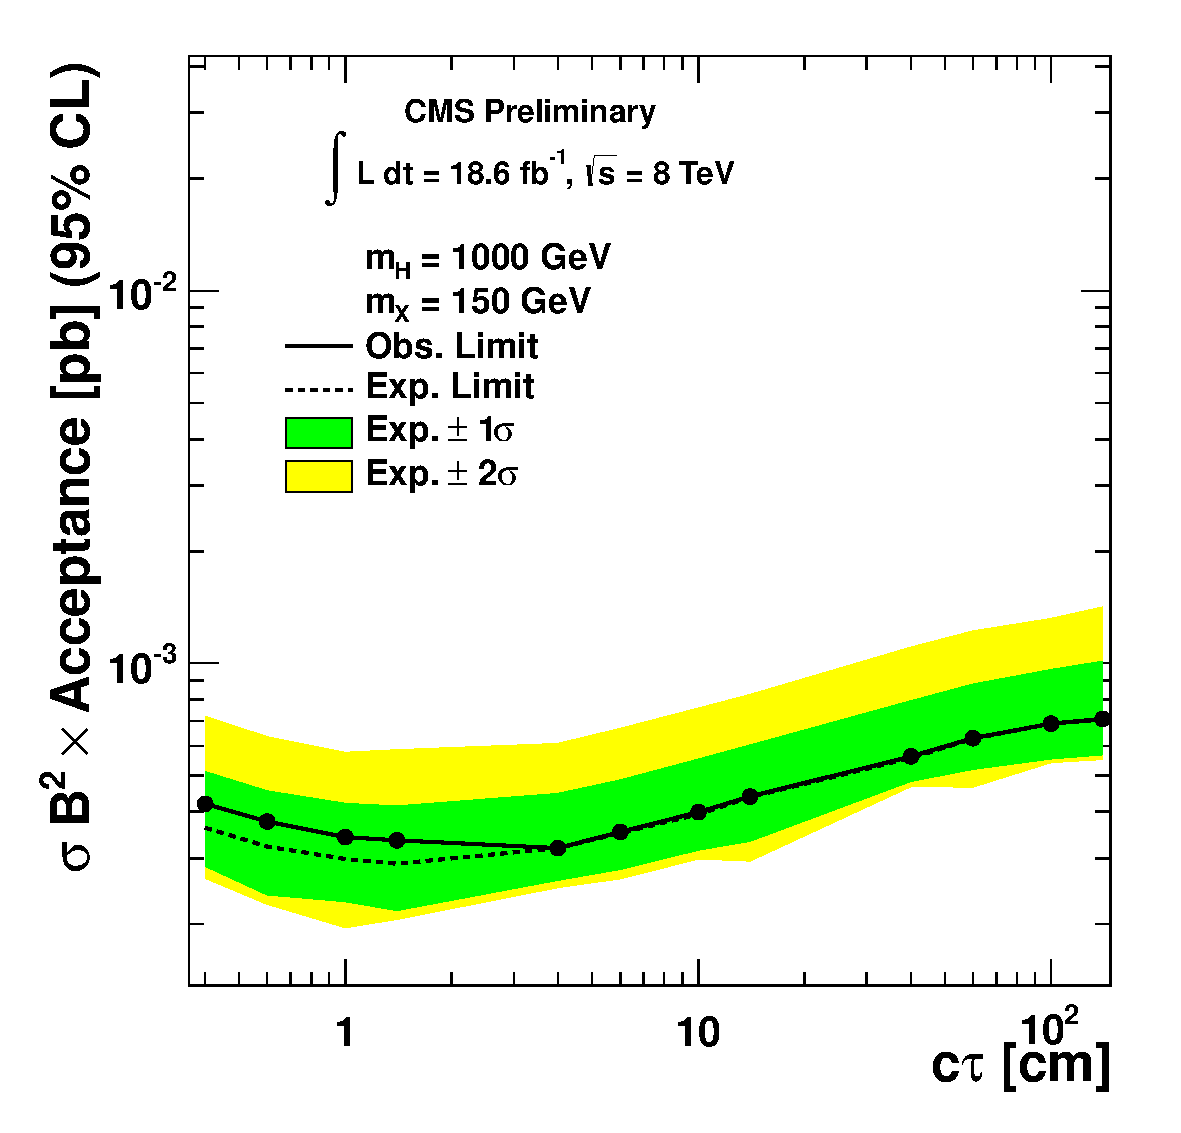
\includegraphics[width=0.49\textwidth]{plots/limits/1000_150ea.pdf} 
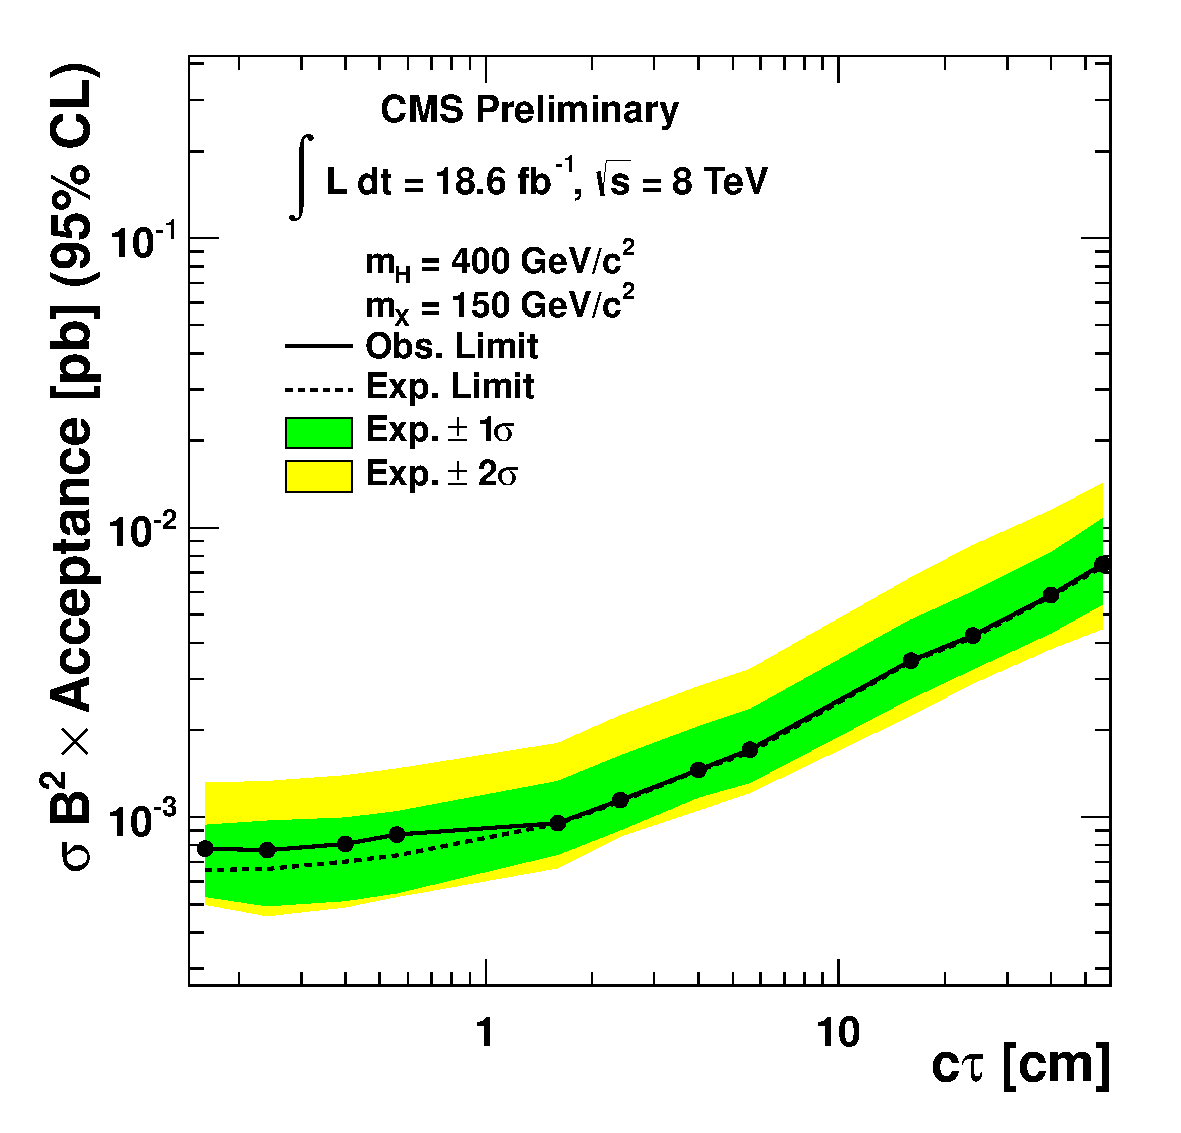
\includegraphics[width=0.49\textwidth]{plots/limits/400_150ea.pdf}
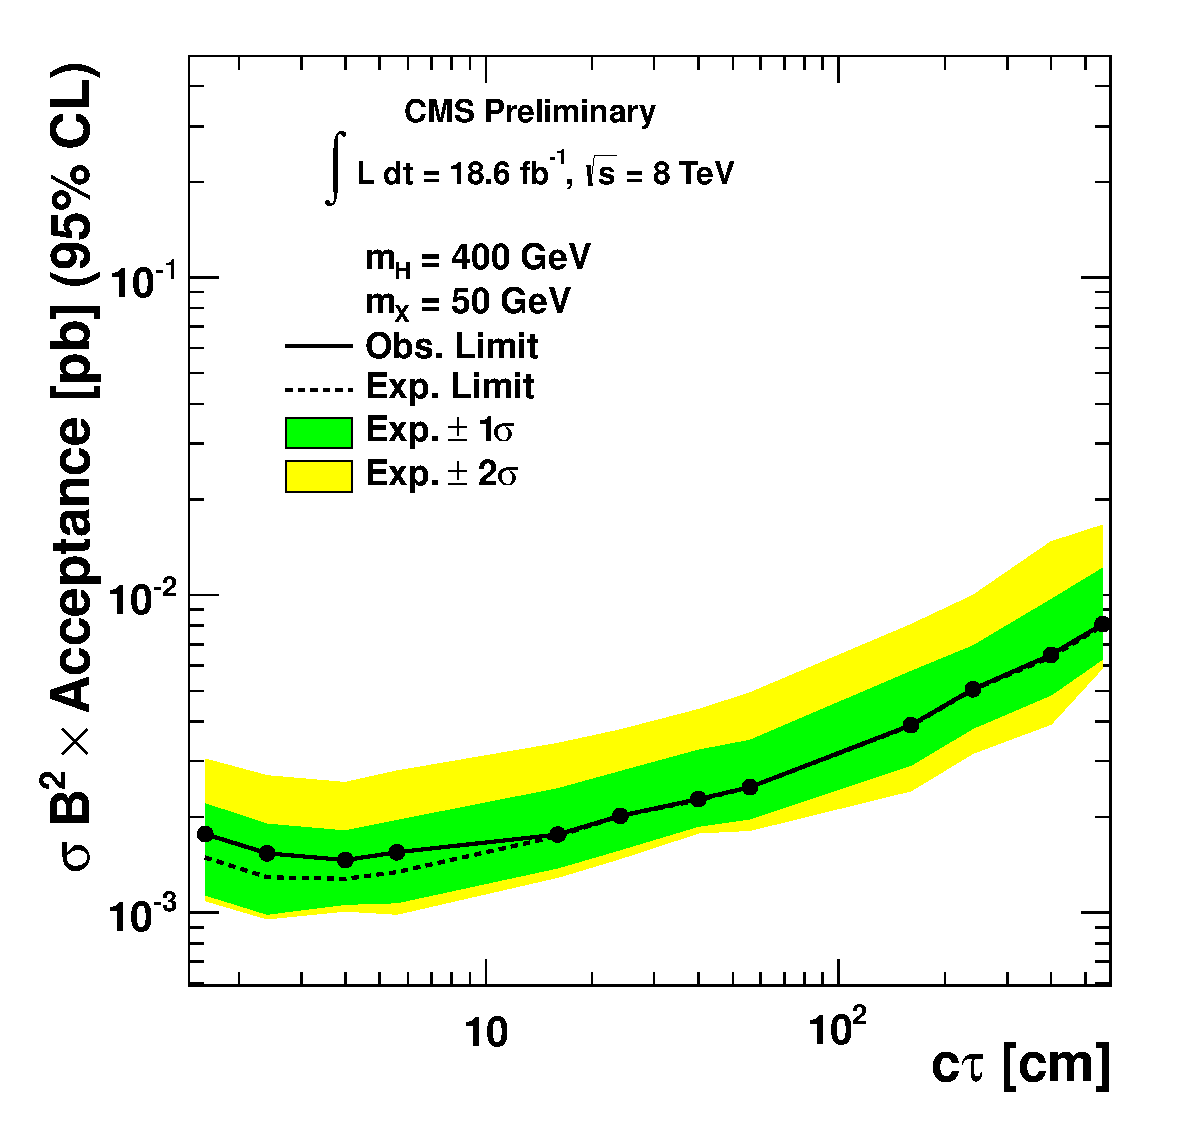
\includegraphics[width=0.49\textwidth]{plots/limits/400_50ea.pdf} 
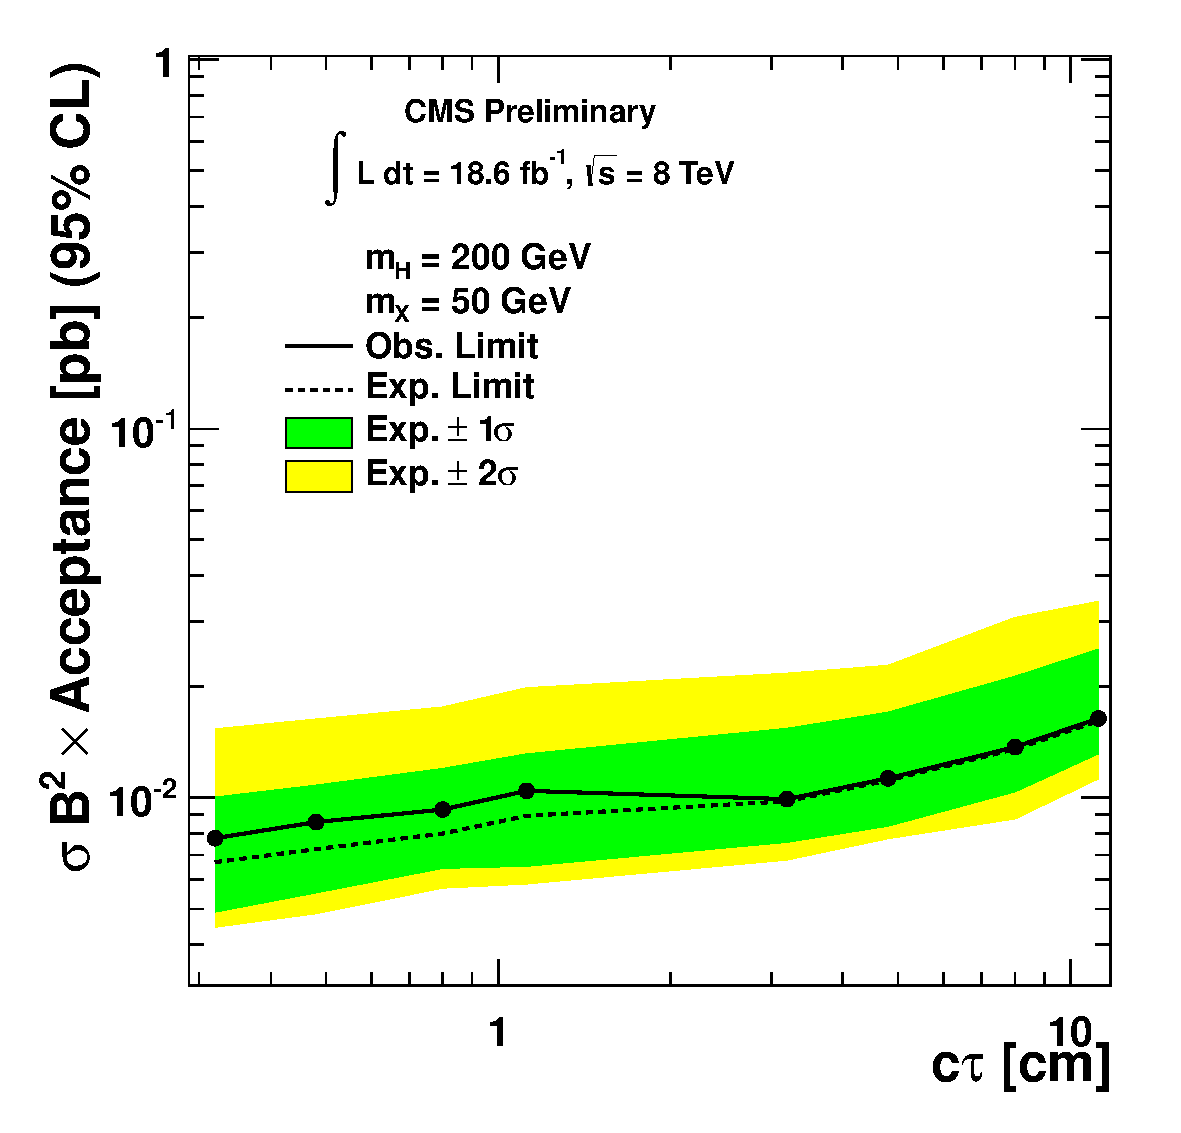
\includegraphics[width=0.49\textwidth]{plots/limits/200_50ea.pdf}

\caption{Expected and observed 95\% CL limits within the detector acceptance for all tested signal models.\label{fig:limitsacceptance}}
\end{figure}

\subsection{Conclusions}
\label{subsec:conclusions}

For pp collisions at $\sqrt{s}=8 \TeV$, upper limits are placed on the production cross section
of a heavy resonance decaying to two long-lived, spin 0, neutral particles \X, where the massive resonance
is taken to be a Higgs boson, times the branching ratio squared of $\X$ decaying to \qq, where $q$ denotes any
of the $u,d,s,c,b$ quark flavors. For Higgs masses of 200-1000\GeVcc and \X boson masses of 50-350\GeVcc,
these limits are typically in the range 0.0005-0.3 $pb$, for \X bosons whose lifetime is such their mean 
transverse decay length is less than about 1 metre.     
